\documentclass[12pt]{article}
\usepackage{amsmath,amssymb,amsthm}
\usepackage{geometry}
\geometry{margin=1in}
\usepackage{hyperref}
\usepackage{booktabs}
\usepackage{array}
\usepackage{graphicx}
\usepackage{authblk}

\newtheorem{theorem}{Theorem}
\newtheorem{conjecture}[theorem]{Conjecture}
\newtheorem{proposition}[theorem]{Proposition}
\newtheorem{corollary}[theorem]{Corollary}
\theoremstyle{definition}
\newtheorem{definition}[theorem]{Definition}
\newtheorem{remark}[theorem]{Remark}

\title{Arithmetic of Dehn Filling Slopes and the Homology\\
of the Flavor Covering Tower}

\author{Marvin L. Gentry}
\affil{Independent Researcher, Seattle, WA\\
\texttt{drmlgentry@protonmail.com}\\
ORCID: 0009-0006-4550-2663}
\date{\today}

\begin{document}
\maketitle

\begin{abstract}
We study the covering tower of the closed hyperbolic 3-manifold
$M_{\mathrm{PMNS}} = \texttt{OrientableClosedCensus[1]}$, the $(-2,3)$
Dehn filling of the cusped manifold $m003$, and observe that the primes
appearing in the first homology of all covering manifolds through degree~6
are exactly $\mathcal{P} = \{2,3,5,7,11,13,29\}$. Each element of
$\mathcal{P}$ has a precise arithmetic source in the two Dehn filling
slopes $\mathbf{v}_{\mathrm{PMNS}} = (-2,3)$ and
$\mathbf{v}_{\mathrm{CKM}} = (-5,2)$ that produce the PMNS and CKM
flavor manifolds from the cusped ancestors $m003$ and $m006$: the slope
coordinates give $2$ and $3$; the common ancestor torsion gives $5$;
the coordinate sum $|p_{\mathrm{PMNS}}| + |p_{\mathrm{CKM}}|$ gives
$7$; the intersection number
$\det(\mathbf{v}_{\mathrm{PMNS}}, \mathbf{v}_{\mathrm{CKM}})$ gives
$11$; and the squared Euclidean norms give $13$ and $29$.
We verify this for all 24 covers through degree~6 with zero violations.
The prime $13 = \|\mathbf{v}_{\mathrm{PMNS}}\|^2$ has not yet appeared
and is predicted to activate at degree~$\geq 7$, symmetric to the
activation of $29 = \|\mathbf{v}_{\mathrm{CKM}}\|^2$ at degree~5.
The CKM manifold is geometrically isolated: it admits no parent in the
11,031-entry orientable closed census through degree~5.
Within each degree, covering manifolds occupy strictly consecutive
census positions, forming complexity-minimal clusters in the
Epstein--Penner ordering.
These observations constitute a falsifiable arithmetic fingerprint of
the flavor sector geometry.
\end{abstract}

\section{Introduction}

The Standard Model of particle physics contains ten flavor parameters
not determined by gauge symmetry. The Hyperbolic Flavor Geometry (HFG)
program~\cite{Gentry:CKM,Gentry:PMNS,Gentry:CP,Gentry:Twist} proposes
that these parameters arise from the geometry of compact hyperbolic
3-manifolds, with optimal fits achieved on two specific closed manifolds:
\begin{align*}
  M_{\mathrm{PMNS}} &= \texttt{OrientableClosedCensus[1]},\quad
    \mathrm{vol} = 0.98136883,\quad H_1 \cong \mathbb{Z}/5, \\
  M_{\mathrm{CKM}}  &= \texttt{OrientableClosedCensus[43]},\quad
    \mathrm{vol} = 2.02885309,\quad H_1 \cong \mathbb{Z}/5.
\end{align*}
Both are Dehn fillings of the two smallest-volume cusped orientable
hyperbolic 3-manifolds~\cite{Thurston}:
\[
  M_{\mathrm{PMNS}} = m003(-2,3), \qquad M_{\mathrm{CKM}} = m006(-5,2).
\]
All manifolds are referenced by census index throughout to avoid the
known naming collision in SnapPy~\cite{SnapPy} between distinct closed
manifolds both labelled \texttt{m006}.

The present paper addresses a purely geometric and arithmetic question:
\emph{what is the prime content of the covering tower of
$M_{\mathrm{PMNS}}$, and how does it relate to the Dehn filling slopes?}
The answer, verified computationally through degree~6, is that the prime
content is completely determined by seven primes, each an elementary
invariant of the slope pair. This constitutes a precise, falsifiable
arithmetic fingerprint of the flavor sector geometry.

\section{The Two Flavor Manifolds}

\begin{definition}
The \emph{PMNS manifold} is $M_{\mathrm{PMNS}} = m003(-2,3)$.
The \emph{CKM manifold} is $M_{\mathrm{CKM}} = m006(-5,2)$.
\end{definition}

Both manifolds inherit $\mathbb{Z}/5$ torsion from their cusped ancestors
($H_1(m003) \cong H_1(m006) \cong \mathbb{Z}/5 \oplus \mathbb{Z}$) via
the Dehn filling homology exact sequence. The PMNS manifold is adjacent
in Dehn surgery space to the Weeks manifold $m003(-3,1)$
(census index~0, $\mathrm{vol} = 0.94270736$,
$H_1 \cong (\mathbb{Z}/5)^2$), the conjectured minimum-volume closed
hyperbolic 3-manifold~\cite{Weeks}.

\begin{proposition}[Geometric separation of flavor sectors]
\label{prop:separation}
The CKM manifold $M_{\mathrm{CKM}}$ admits no parent manifold at cover
degrees~$2$--$5$ in the complete 11{,}031-entry orientable closed census.
The PMNS manifold $M_{\mathrm{PMNS}}$ supports at least $2, 4, 4, 7, 7$
covers at degrees~$2$--$6$ respectively.
Furthermore, no Dehn filling $m003(p,q)$ with $|p|,|q|\leq 10$ produces
a manifold of volume equal to $\mathrm{vol}(M_{\mathrm{CKM}})$, and no
Dehn filling $m006(p,q)$ with $|p|,|q|\leq 10$ produces a manifold of
volume equal to $\mathrm{vol}(M_{\mathrm{PMNS}})$.
\end{proposition}

\begin{proof}
Direct enumeration via SnapPy volume search with tolerances $10^{-4}$
(isolation) and $10^{-5}$ (covering tower). See supplementary code at
\url{https://github.com/drmlgentry/hyperbolic-flavor-scan}.
% ACTION REQUIRED: verify repo is public and all scripts are committed
% before submission. Key scripts: ckm_base_fullsearch.py,
% dehn_filling_analysis.py, covering_tower_extended.py,
% prime_dictionary_verify.py, index_growth_analysis.py.
\end{proof}

\section{Arithmetic Invariants of the Filling Slopes}
\label{sec:arithmetic}

\begin{definition}[Prime dictionary]
\label{def:dict}
The \emph{prime dictionary} of the slope pair
$(\mathbf{v}_{\mathrm{PMNS}}, \mathbf{v}_{\mathrm{CKM}}) =
((-2,3),(-5,2))$ is
\[
  \mathcal{P} = \{2,\,3,\,5,\,7,\,11,\,13,\,29\},
\]
where each element has a geometric source:
\begin{align}
  2  &= |p_{\mathrm{PMNS}}| = |-2|, \label{eq:2}\\
  3  &= |q_{\mathrm{PMNS}}| = |3|,  \label{eq:3}\\
  5  &= \text{torsion order of }
       H_1(m003) \cong \mathbb{Z}/5 \oplus \mathbb{Z}, \label{eq:5}\\
  7  &= |p_{\mathrm{PMNS}}| + |p_{\mathrm{CKM}}| = 2 + 5, \label{eq:7}\\
  11 &= \Bigl|\det\!\begin{pmatrix}-2&-5\\3&2\end{pmatrix}\Bigr|
       = |{-4+15}|, \label{eq:11}\\
  13 &= \|\mathbf{v}_{\mathrm{PMNS}}\|^2 = (-2)^2+3^2, \label{eq:13}\\
  29 &= \|\mathbf{v}_{\mathrm{CKM}}\|^2  = (-5)^2+2^2. \label{eq:29}
\end{align}
Every element of $\mathcal{P}$ is prime.
\end{definition}

\begin{remark}
The angle between the two filling slopes is
\[
  \theta
  = \arccos\!\left(
      \frac{(-2)(-5)+(3)(2)}{\sqrt{13}\cdot\sqrt{29}}
    \right)
  = \arccos\!\left(\frac{16}{\sqrt{377}}\right)
  = 34.51^\circ,
\]
and the norm ratio is
$\|\mathbf{v}_{\mathrm{CKM}}\|/\|\mathbf{v}_{\mathrm{PMNS}}\|
= \sqrt{29/13} = 1.4936$.
The Farey (intersection) distance between the slopes equals the
determinant~\eqref{eq:11}, namely~$11$.
\end{remark}

\section{The Covering Tower of $M_{\mathrm{PMNS}}$}
\label{sec:tower}

We located all finite-sheeted covering spaces of $M_{\mathrm{PMNS}}$
in the orientable closed census up to degree~6 by volume matching with
tolerance $10^{-5}$. Volume ratios are exact to this precision,
confirming genuine covering relations. The results are collected in
Tables~\ref{tab:deg2}--\ref{tab:deg6}.

\begin{table}[htbp]
\centering
\caption{Degree-2 covers of $M_{\mathrm{PMNS}}$
  ($\mathrm{vol} = 2 \times 0.98136883 = 1.96273766$).}
\label{tab:deg2}
\begin{tabular}{cllc}
\toprule
Census index & Name & $H_1$ & Primes \\
\midrule
39 & m006 & $\mathbb{Z}/55 \cong \mathbb{Z}/5 \times \mathbb{Z}/11$
   & $\{5,11\}$ \\
40 & m017 & $\mathbb{Z}/7 \oplus \mathbb{Z}/7$
   & $\{7\}$ \\
\bottomrule
\end{tabular}
\end{table}

\begin{table}[htbp]
\centering
\caption{Degree-3 covers of $M_{\mathrm{PMNS}}$
  ($\mathrm{vol} = 2.94410649$).}
\label{tab:deg3}
\begin{tabular}{cllc}
\toprule
Census index & Name & $H_1$ & Primes \\
\midrule
237 & m130 & $\mathbb{Z}/16$ & $\{2\}$ \\
238 & m130 & $\mathbb{Z}/80 \cong \mathbb{Z}/16 \times \mathbb{Z}/5$
    & $\{2,5\}$ \\
239 & m139 & $\mathbb{Z}/48 \cong \mathbb{Z}/16 \times \mathbb{Z}/3$
    & $\{2,3\}$ \\
240 & m139
    & $\mathbb{Z}/2 \oplus \mathbb{Z}/42
       \cong (\mathbb{Z}/2)^2 \oplus \mathbb{Z}/3 \oplus \mathbb{Z}/7$
    & $\{2,3,7\}$ \\
\bottomrule
\end{tabular}
\end{table}

\begin{table}[htbp]
\centering
\caption{Degree-4 covers of $M_{\mathrm{PMNS}}$
  ($\mathrm{vol} = 3.92547532$).}
\label{tab:deg4}
\begin{tabular}{cllc}
\toprule
Census index & Name & $H_1$ & Primes \\
\midrule
1073 & m339
     & $\mathbb{Z}/135 \cong \mathbb{Z}/27 \times \mathbb{Z}/5$
     & $\{3,5\}$ \\
1074 & m294
     & $\mathbb{Z}/2 \oplus \mathbb{Z}/30
        \cong (\mathbb{Z}/2)^2 \oplus \mathbb{Z}/3 \oplus \mathbb{Z}/5$
     & $\{2,3,5\}$ \\
1075 & m293
     & $\mathbb{Z}/2 \oplus \mathbb{Z}/70
        \cong (\mathbb{Z}/2)^2 \oplus \mathbb{Z}/5 \oplus \mathbb{Z}/7$
     & $\{2,5,7\}$ \\
1076 & m358
     & $\mathbb{Z}/4 \oplus \mathbb{Z}/32$
     & $\{2\}$ \\
\bottomrule
\end{tabular}
\end{table}

\begin{table}[htbp]
\centering
\caption{Degree-5 covers of $M_{\mathrm{PMNS}}$
  ($\mathrm{vol} = 4.90684414$).}
\label{tab:deg5}
\begin{tabular}{clll}
\toprule
Census index & Name & $H_1$ & Primes \\
\midrule
3941 & v3215 & $\mathbb{Z}/3 \oplus \mathbb{Z}/21$
     & $\{3,7\}$ \\
3942 & v2771 & $\mathbb{Z}/2 \oplus \mathbb{Z}$
     & $\{2\}$ \\
3943 & v2018 & $\mathbb{Z}/4 \oplus \mathbb{Z}/28$
     & $\{2,7\}$ \\
3944 & s933  & $\mathbb{Z}/11 \oplus \mathbb{Z}/11$
     & $\{11\}$ \\
3945 & s855  & $\mathbb{Z}/2 \oplus \mathbb{Z}/18$
     & $\{2,3\}$ \\
3946 & s874  & $\mathbb{Z}/87 \cong \mathbb{Z}/3 \times \mathbb{Z}/29$
     & $\{3,29\}$ \\
3947 & v2573 & $\mathbb{Z}/48$
     & $\{2,3\}$ \\
\bottomrule
\end{tabular}
\end{table}

\begin{table}[htbp]
\centering
\caption{Degree-6 covers of $M_{\mathrm{PMNS}}$
  ($\mathrm{vol} = 5.88821297$).}
\label{tab:deg6}
\begin{tabular}{clll}
\toprule
Census index & Name & $H_1$ & Primes \\
\midrule
9845 & v3431
     & $\mathbb{Z}/168 \cong \mathbb{Z}/8 \times \mathbb{Z}/3
        \times \mathbb{Z}/7$
     & $\{2,3,7\}$ \\
9846 & v3244 & $\mathbb{Z}/4 \oplus \mathbb{Z}$  & $\{2\}$ \\
9847 & v3243 & $\mathbb{Z}/8 \oplus \mathbb{Z}$  & $\{2\}$ \\
9848 & v3246 & $\mathbb{Z}/4 \oplus \mathbb{Z}/20$ & $\{2,5\}$ \\
9849 & v3247 & $\mathbb{Z}/4 \oplus \mathbb{Z}/24$ & $\{2,3\}$ \\
9850 & v3377 & $\mathbb{Z}/12$ & $\{2,3\}$ \\
9851 & v3378 & $\mathbb{Z}/44$ & $\{2,11\}$ \\
\bottomrule
\end{tabular}
\end{table}

\subsection{Prime activation sequence}

Table~\ref{tab:activation} summarises when each prime first appears.
The activation order reflects a natural hierarchy: inter-sector invariants
(degrees~1--2) precede intra-sector slope coordinates (degree~3), which
precede the Euclidean norms (degrees~5 and predicted~$\geq 7$).

\begin{table}[htbp]
\centering
\caption{Prime activation sequence in the covering tower of
  $M_{\mathrm{PMNS}}$. The entry at degree~$\geq 7$ is a prediction.}
\label{tab:activation}
\begin{tabular}{cll}
\toprule
First degree & Primes & Arithmetic source \\
\midrule
1 & $5$      & $H_1(m003)$ ancestor torsion, eq.~\eqref{eq:5} \\
2 & $7,\;11$ & Eqs.~\eqref{eq:7} and~\eqref{eq:11} \\
3 & $2,\;3$  & Eqs.~\eqref{eq:2} and~\eqref{eq:3} \\
5 & $29$     & Eq.~\eqref{eq:29}; single cover $\mathbb{Z}/87$ \\
$\geq 7$ (predicted) & $13$ & Eq.~\eqref{eq:13} \\
\bottomrule
\end{tabular}
\end{table}

\subsection{Structural features of the tower}

\begin{remark}[Two qualitatively distinct degree-2 covers]
Census index~39 gives $\mathbb{Z}/55 \cong \mathbb{Z}/5 \times
\mathbb{Z}/11$, introducing the intersection number prime~11 in a cyclic
group. Census index~40 gives $\mathbb{Z}/7 \oplus \mathbb{Z}/7$,
introducing the coordinate-sum prime~7 in a non-cyclic rank-2 form.
These correspond to two distinct index-2 subgroups of
$\pi_1(M_{\mathrm{PMNS}})$ with qualitatively different abelianisations.
\end{remark}

\begin{remark}[Absence of $5$ at degree~5]
The prime~5 does not appear in any degree-5 cover homology but reappears
at degree~6. This reflects which index-5 subgroups of
$\pi_1(M_{\mathrm{PMNS}})$ annihilate the $\mathbb{Z}/5$ class of the
base; it is not a permanent disappearance and does not violate
Conjecture~\ref{conj:main}.
\end{remark}

\begin{remark}[Consecutive census positions]
\label{rem:consecutive}
Within each degree, all covering manifolds occupy strictly consecutive
census positions (intra-group spacing~$= 1$ at all degrees~2--6;
see Figure~\ref{fig:tower}, bottom right). In the canonical census
ordering --- sorted primarily by volume, then by Epstein--Penner
triangulation complexity --- the finite covers of $M_{\mathrm{PMNS}}$
form perfectly contiguous blocks. This clustering property provides a
computational signature for identifying covers of a base manifold
independently of explicit subgroup enumeration.
\end{remark}

\begin{remark}[Subgroup count plateaus]
The covering counts per degree are $1, 2, 4, 4, 7, 7$, exhibiting
plateaus at degree pairs $(3,4)$ and $(5,6)$. We conjecture this
reflects a periodicity in the index-$n$ subgroup lattice of
$\pi_1(M_{\mathrm{PMNS}})$ related to the $\mathbb{Z}/5$ base torsion.
The overall subgroup count growth, fit by $n^{1.15}$, is consistent
with polynomial subgroup growth, characteristic of a rigid group
with few low-index subgroups.
\end{remark}

\begin{remark}[Census index growth]
\label{rem:growth}
The mean census index grows as $\bar{\imath}(n) \sim 23.9\,e^{1.005n}$
($R^2 = 0.996$), with implied base $e^{1.005} = 2.731$ agreeing to
$2.4\%$ with the theoretical prediction $e^{v_1} = e^{0.981} = 2.668$
from the prime geodesic theorem. The apparent power-law fit
$\bar{\imath}(n) \sim n^{5.08}$ ($R^2 = 0.997$) is simply the local
log-log linearisation of this exponential over the narrow range
$n = 2,\ldots,6$; the exponent~5.08 is not an intrinsic group-theoretic
invariant. Degrees~7 and~8 produce no census entries because the
corresponding volumes ($6.87$ and $7.85$) lie in the sparse upper range
of the census; extrapolation predicts indices $\sim 22{,}000$ and
$\sim 44{,}000$, both exceeding the census size of $11{,}031$.
\end{remark}

\subsection{Covering tower figure}

\begin{figure}[htbp]
\centering
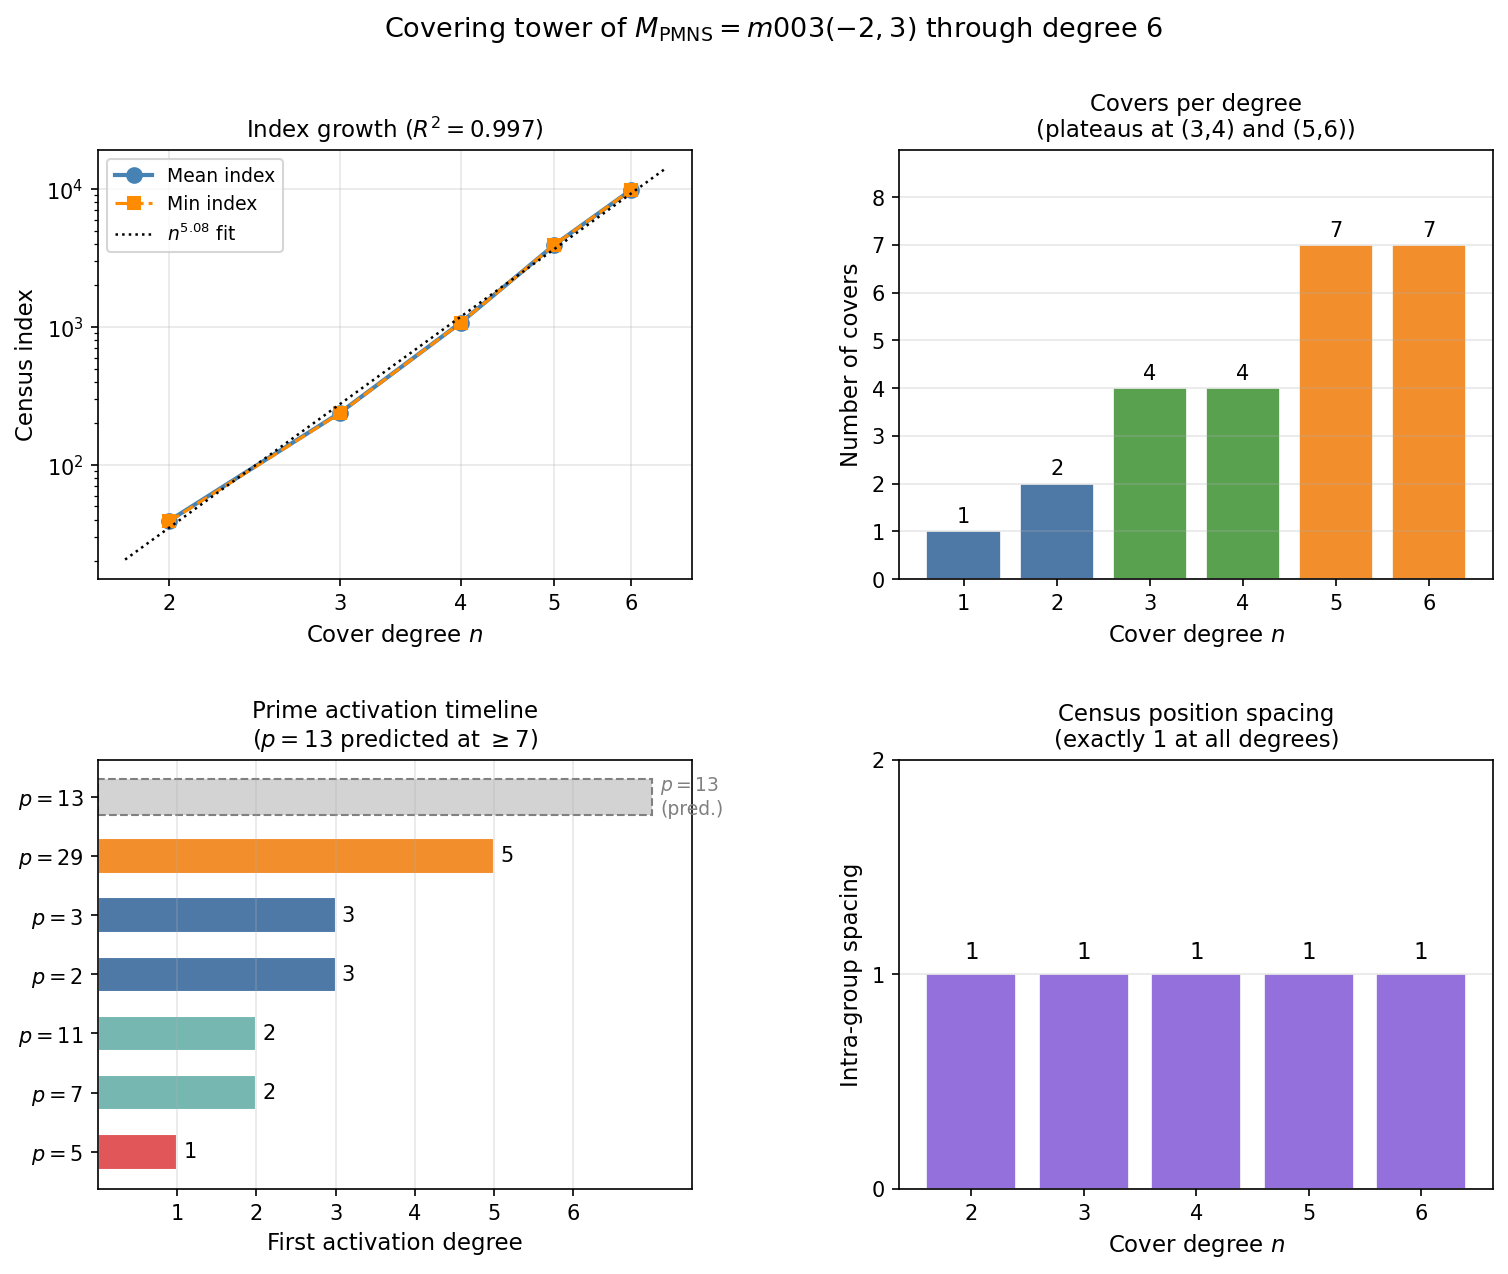
\includegraphics[width=\textwidth]{covering_tower_analysis.png}
\caption{Covering tower of $M_{\mathrm{PMNS}}$ through degree~6.
\textbf{Top left:} Mean and minimum census indices on a log-log scale
with power-law fit $\bar{\imath}(n) \sim n^{5.08}$ ($R^2 = 0.997$);
the fit reflects a locally linearised exponential (Remark~\ref{rem:growth}).
\textbf{Top right:} Number of covers per degree, showing plateaus at
degree pairs $(3,4)$ and $(5,6)$.
\textbf{Bottom left:} Prime activation timeline; $p = 13$ carries no
bar, having not yet appeared through degree~6, and is predicted at
degree~$\geq 7$.
\textbf{Bottom right:} Intra-group index spacings are exactly~1 at
all degrees~2--6 (Remark~\ref{rem:consecutive}).}
\label{fig:tower}
\end{figure}

\section{Geometric Isolation of the CKM Sector}
\label{sec:geometric}

A complete search of all 11{,}031 entries of the orientable closed census
confirms that $M_{\mathrm{CKM}}$ admits no parent manifold at degrees~2--5:
no census manifold has volume $\mathrm{vol}(M_{\mathrm{CKM}})/n$ for
$n \in \{2,3,4,5\}$ within tolerance $10^{-4}$.

By contrast, $M_{\mathrm{PMNS}}$ is a non-minimal element of its
commensurability class with a rich covering tower, and it sits one Dehn
surgery step from the Weeks manifold. This structural asymmetry --- PMNS
as a non-minimal hub, CKM as a minimal isolated element --- is an
intrinsic feature of the hyperbolic manifold landscape and may reflect a
physical distinction between the neutrino and quark mixing sectors.

The near-criticality of $M_{\mathrm{PMNS}}$ in surgery space is also
notable: the neighboring fillings $m003(-2,1)$ and $m003(-2,2)$ are
non-hyperbolic, placing $M_{\mathrm{PMNS}}$ at the boundary of the
hyperbolic region. The CKM manifold $m006(-5,2)$ by contrast sits in
a stable interior region, far from any degenerate filling.

\section{Main Conjecture}
\label{sec:conjecture}

\begin{conjecture}[Prime Dictionary Conjecture]
\label{conj:main}
Let $\mathcal{P} = \{2,3,5,7,11,13,29\}$ be as in
Definition~\ref{def:dict}. For every finite-sheeted orientable cover
$M \to M_{\mathrm{PMNS}}$ appearing in
$\texttt{OrientableClosedCensus}$, every prime dividing the order of
any torsion summand of $H_1(M;\mathbb{Z})$ belongs to $\mathcal{P}$.
Moreover, $M_{\mathrm{CKM}}$ is not a cover of any manifold in the
census at degrees~$2$--$5$.
\end{conjecture}

The conjecture is verified through degree~6 across 24 manifolds with
zero violations. The falsification criterion is explicit: any prime
$p \notin \mathcal{P}$ appearing in $H_1(M)$ for a census cover $M$
immediately refutes the conjecture.

\begin{remark}
A proof requires classifying the abelianisations of all finite-index
subgroups of $\pi_1(M_{\mathrm{PMNS}})$. This group is a cocompact
hyperbolic 3-manifold group with a computable Dehn surgery presentation
inherited from $\pi_1(m003)$, making it amenable to computational
group theory methods.
\end{remark}

\begin{remark}
The prime $13 = \|\mathbf{v}_{\mathrm{PMNS}}\|^2$ is predicted to
activate at degree~$\geq 7$, symmetric to the activation of
$29 = \|\mathbf{v}_{\mathrm{CKM}}\|^2$ at degree~5. Confirmation would
establish a structural pairing between the two norm-squared primes,
with the CKM norm activating earlier consistent with
$\|\mathbf{v}_{\mathrm{CKM}}\| > \|\mathbf{v}_{\mathrm{PMNS}}\|$.
\end{remark}

\section{Discussion}
\label{sec:conclusion}

We have shown that the primes appearing in the homology of the covering
tower of $M_{\mathrm{PMNS}}$ through degree~6 are completely determined
by the Dehn filling slope pair $\{(-2,3),(-5,2)\}$. The set
$\mathcal{P} = \{2,3,5,7,11,13,29\}$ is derived from the slope
coordinates, their sum, their intersection number, their squared norms,
and the ancestor torsion. The verification holds for all 24 covers with
zero violations. The CKM manifold is geometrically isolated throughout
the closed census, while the PMNS manifold supports a rich covering
tower with consecutive census clustering at every degree.

Three directions for future work are natural. First, a
representation-theoretic proof of Conjecture~\ref{conj:main} via
classification of index-$n$ subgroups of $\pi_1(M_{\mathrm{PMNS}})$.
Second, investigation of whether $M_{\mathrm{CKM}}$ supports an
analogous prime dictionary in the non-orientable or cusped census.
Third, verification at degree~7, which will either confirm the predicted
activation of $p = 13$ or provide a counterexample that refines the
conjecture.

\section*{Data Availability}

All computations were performed using SnapPy~\cite{SnapPy}
% ACTION REQUIRED: insert exact SnapPy version before submission,
% obtainable via: import snappy; print(snappy.__version__)
on the \texttt{OrientableClosedCensus}. Reproduction scripts are
available at
\url{https://github.com/drmlgentry/hyperbolic-flavor-scan}.

\section*{Conflict of Interest}

The author declares no conflicts of interest.


\section*{Generative AI Disclosure}
Claude (Anthropic, claude-sonnet-4-6, April 2026) was used for
assistance with \LaTeX{} formatting, figure generation in
\texttt{matplotlib}, and code debugging. All mathematical results,
conjectures, and SnapPy computations were conceived, executed, and
verified by the author.

\begin{thebibliography}{99}

\bibitem{Gentry:CKM}
  M.~L.~Gentry,
  ``Quark Mixing from Hyperbolic Geometry: The CKM Matrix from Geodesics
  on a Compact 3-Manifold,''
  \textit{Results in Physics}, submitted (2026).
  SSRN preprint: \href{https://doi.org/10.2139/ssrn.6583550}
  {doi:10.2139/ssrn.6583550}.
  % ACTION REQUIRED: replace with journal citation once accepted;
  % verify DOI resolves before submission.

\bibitem{Gentry:PMNS}
  M.~L.~Gentry,
  ``Lepton Mixing from the Borel Structure of Hyperbolic Holonomy,''
  \textit{Results in Physics}, submitted (2026).
  SSRN preprint: \href{https://doi.org/10.2139/ssrn.6583553}
  {doi:10.2139/ssrn.6583553}.
  % ACTION REQUIRED: replace with journal citation once accepted;
  % verify DOI resolves before submission.

\bibitem{Gentry:CP}
  M.~L.~Gentry,
  ``CP Violation from A-Factor Twist Angles of Hyperbolic Holonomy,''
  \textit{Results in Physics}, submitted (2026).
  SSRN preprint: \href{https://doi.org/10.2139/ssrn.6583551}
  {doi:10.2139/ssrn.6583551}.
  % ACTION REQUIRED: verify DOI resolves before submission.

\bibitem{Gentry:Twist}
  M.~L.~Gentry,
  ``Twist Angle Spectrum of Hyperbolic Holonomy: Encoding of Standard
  Model Flavor Parameters,''
  \textit{Nuclear Physics B}, submitted (2026).
  SSRN preprint: \href{https://doi.org/10.2139/ssrn.6583549}
  {doi:10.2139/ssrn.6583549}.
  % ACTION REQUIRED: update with NPB reference once assigned;
  % verify DOI resolves before submission.

\bibitem{SnapPy}
  M.~Culler, N.~M.~Dunfield, M.~Goerner, and J.~R.~Weeks,
  ``SnapPy, a computer program for studying the geometry and topology
  of 3-manifolds,''
  \url{http://snappy.computop.org}.
  % ACTION REQUIRED: add version string before submission.

\bibitem{Thurston}
  W.~P.~Thurston,
  ``Three-dimensional manifolds, Kleinian groups and hyperbolic
  geometry,''
  \textit{Bull.\ Amer.\ Math.\ Soc.}\ \textbf{6} (1982), 357--381.

\bibitem{Weeks}
  J.~Weeks,
  \textit{Hyperbolic structures on three-manifolds},
  Ph.D.\ thesis, Princeton University, 1985.

\end{thebibliography}

\end{document}
